\begin{flushright} {\tiny {\color{gray} benchmark\_crsg12.tex}} \end{flushright}

This benchmark was first presented in Crameri \etal (2012) \cite{crsg12} 
and is also presented in Hillebrand \etal (2014) \cite{hitg14}.
It is designed to test the accuracy of the free surface representation in geodynamics code.

The model box spans $2800\si{\km}$ by $700-1100\si{\km}$ 
(greater model height is necessary when employing sticky air on top). 
The initial condition is specified by a mantle of $600\si{\km}$ thickness, overlain by a cosine shaped, 
$93-107\si{km}$-thick lithosphere:

\begin{center}
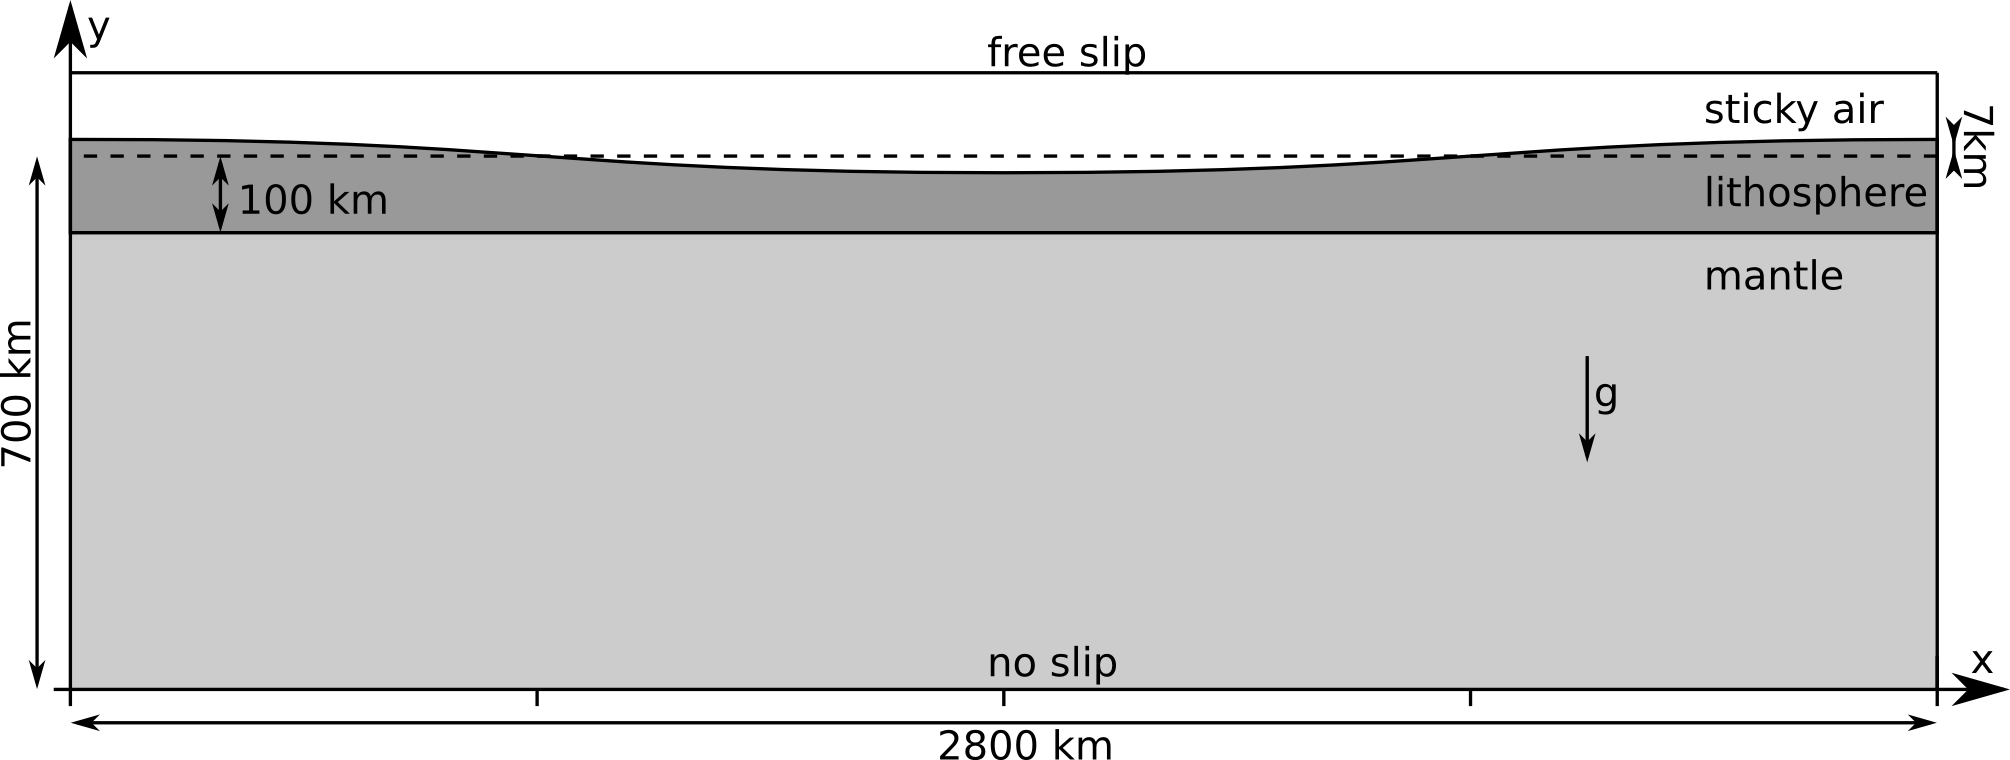
\includegraphics[width=12cm]{images/benchmark_crsg12/setup}
\end{center}

The sticky air layer has a thickness varying between $10$ and $400\si{\km}$. 
The lithosphere is a highly viscous, dense medium 
($\rho_L=3300\si{\kg\per\cubic\metre}$, $\mu_L=10^{23} \si{\pascal\second}$). 
The underlying ambient mantle has a density $\rho_M =3300\si{\kg\per\cubic\metre}$ 
and a viscosity $\mu_M =10^{21}\si{\pascal\second}$. 

\begin{center}
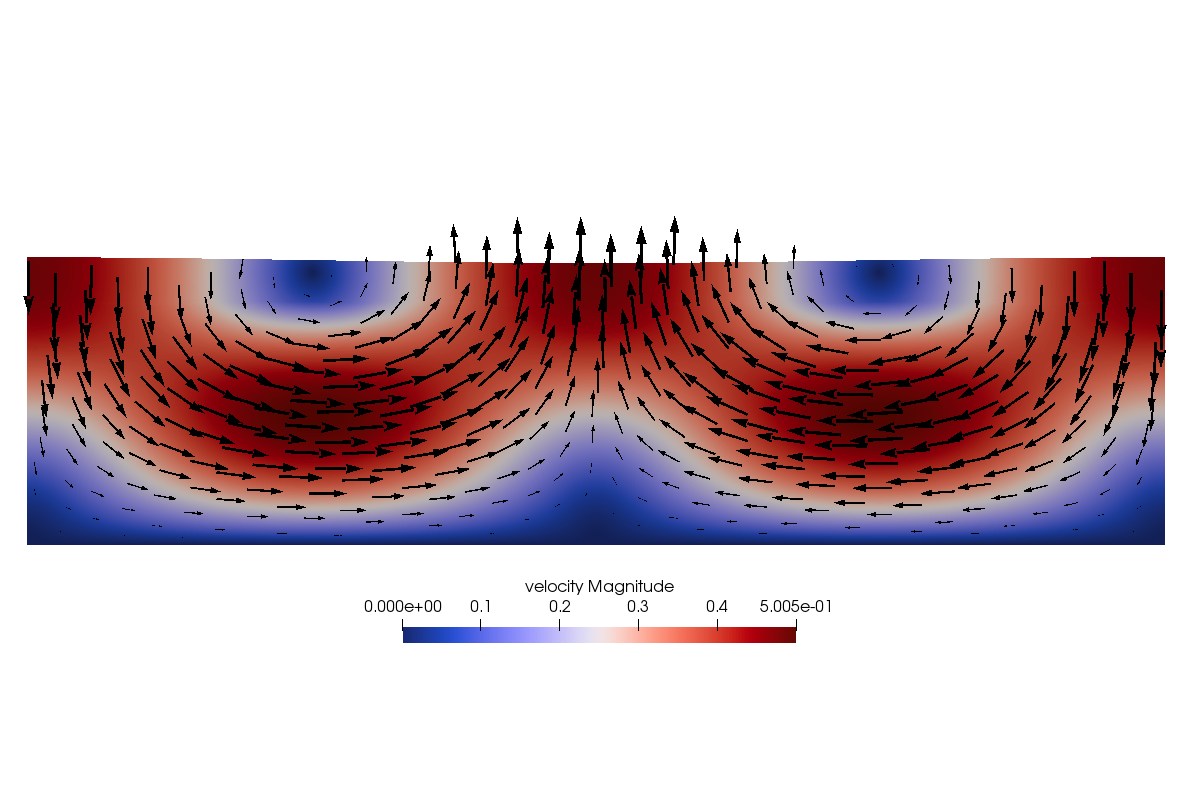
\includegraphics[width=7.5cm]{images/benchmark_crsg12/aspect/vel}
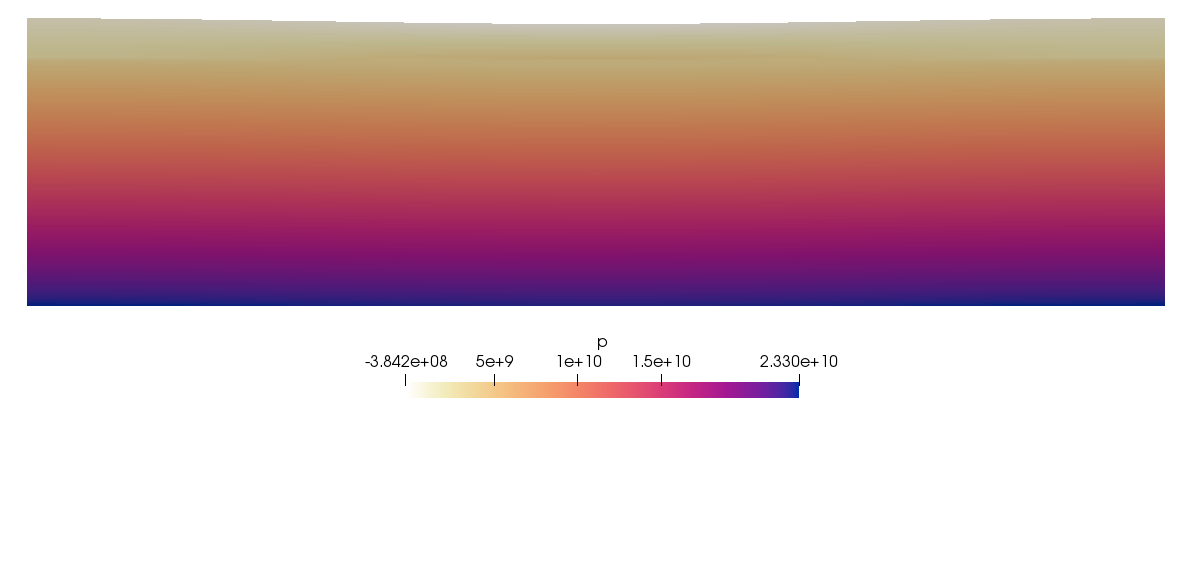
\includegraphics[width=7.5cm]{images/benchmark_crsg12/aspect/press}\\
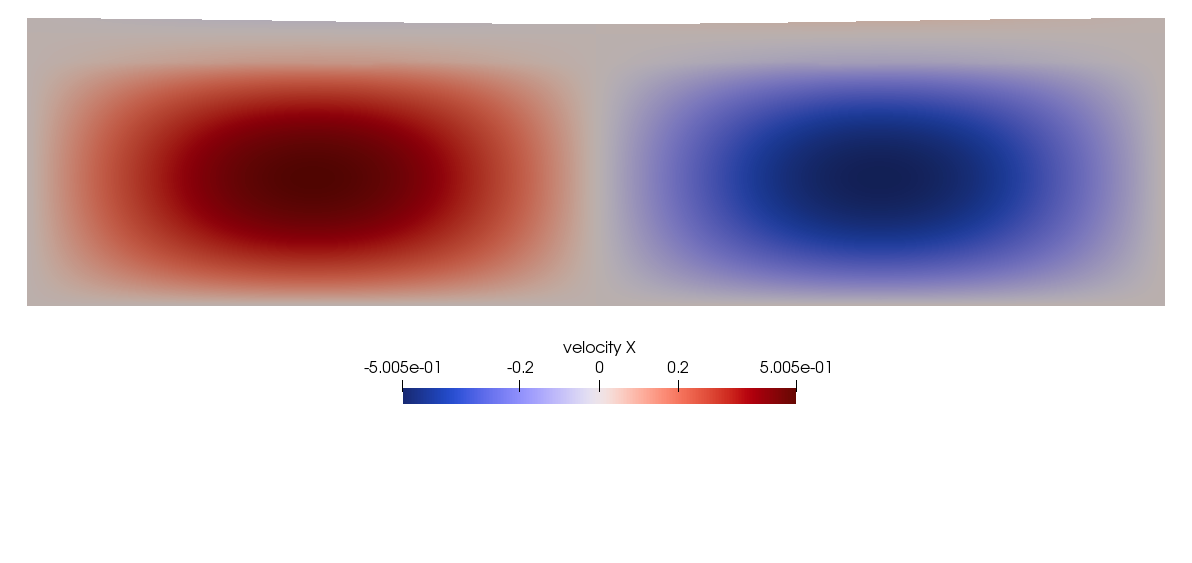
\includegraphics[width=7.5cm]{images/benchmark_crsg12/aspect/u}
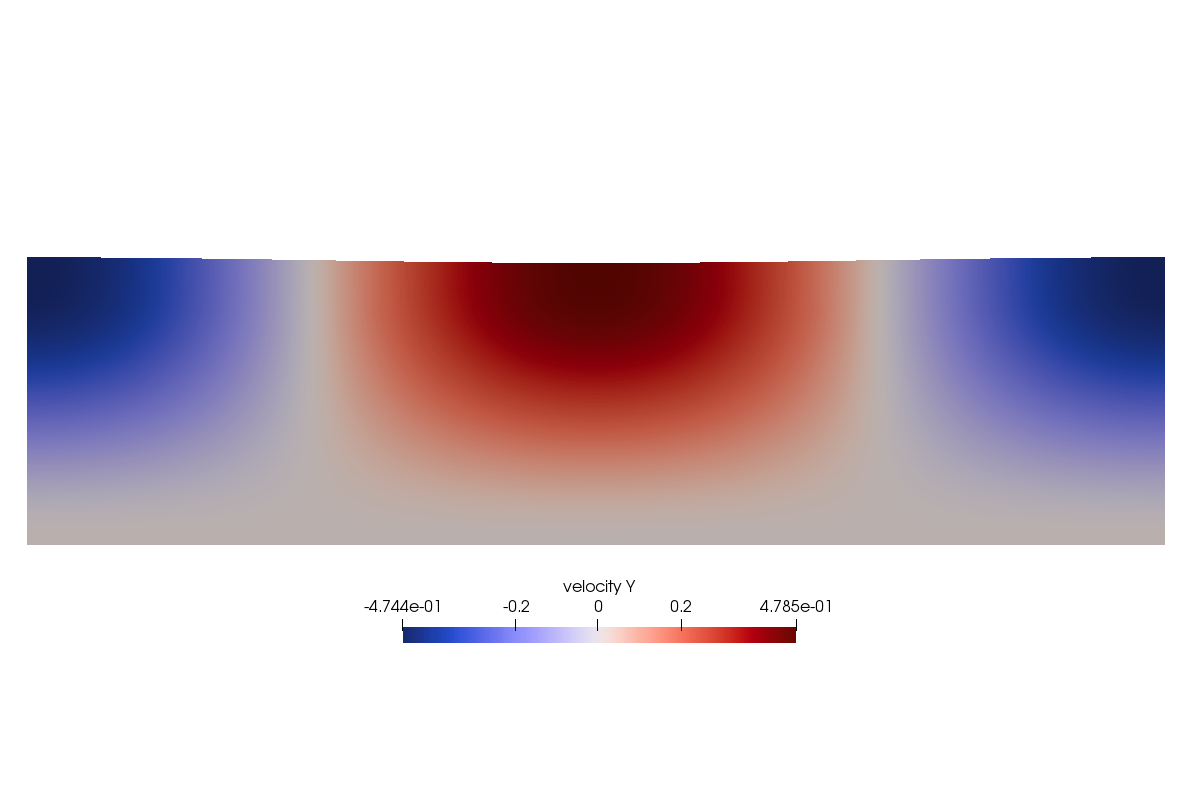
\includegraphics[width=7.5cm]{images/benchmark_crsg12/aspect/v}\\
{\captionfont Results at $t=0$ obtained wirh \aspect{} by running the included cookbook.}
\end{center}


The sticky air layer on the top has a density $\rho_{air} =0\si{\kg\per\cubic\metre}$ 
and a viscosity $\mu_{air} =10^{18}-10^{20}\si{\pascal\second}$ 
and is bordered by a free-slip top boundary condition. 
Free slip is also imposed at the sides while the bottom boundary is set to no slip condition. 

The setup for the real free-surface model is identical to the setup described above, but  
the weak surface layer is removed and replaced by zero normal stress boundary conditions.

An analytical solution is presented by \cite{ramb67}: 
the maximum topography at time $t$ can be derived analytically using the relaxation rate $\gamma$ 
and from the initial maximum topography $h_{init}$:
\begin{equation}
h_{analytic} =h_{init} \exp (\gamma t)
\end{equation}
where $t = 14.825 \si{\kilo\year}$ is the characteristic relaxation 
time and $\gamma = -0.2139 \times 10^{-11} \si{\per\second}$ 
is the characteristic relaxation rate of the three-layer case at a given wavelength of 2800\si{km}. 
It should be noted that these values are valid for infinitesimal amplitudes, 
whereas deviations are to be expected for small but finite amplitudes. In
particular, keeping the interface between the middle and lower layer flat 
and assuming a finite amplitude of the interface between the upper and middle layer 
implies that the thickness of the highly viscous middle layer varies laterally 
by $\pm$7\% (in the case of an initial maximum topography of 7\si{km}). This variation increases the 
effective viscous flexural rigidity and leads to a slightly longer relaxation time.
The system is let to relax over time (typically 200kyrs) and the position of the 
free surface at $x=0$ is recorded over time.

\begin{center}
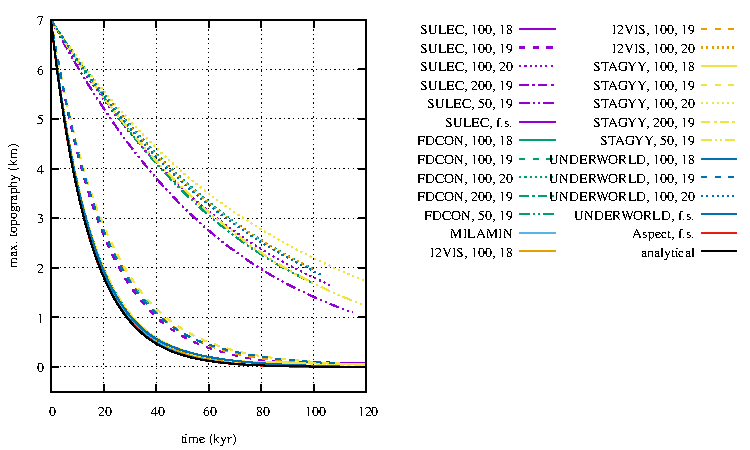
\includegraphics[width=7.5cm]{images/benchmark_crsg12/topo.pdf}
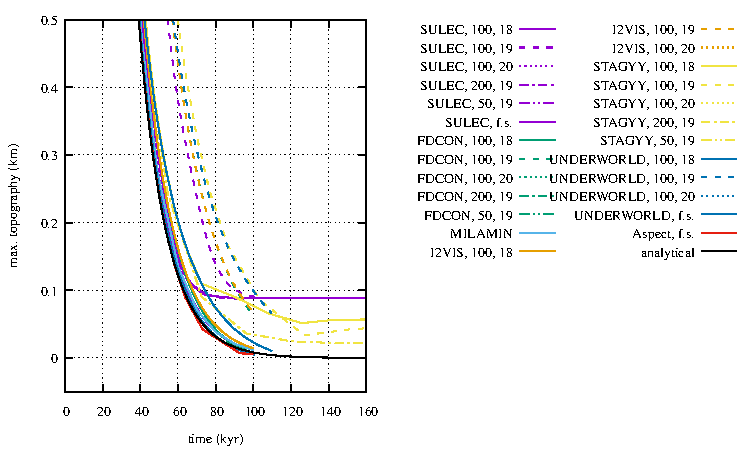
\includegraphics[width=7.5cm]{images/benchmark_crsg12/topozoom.pdf}\\
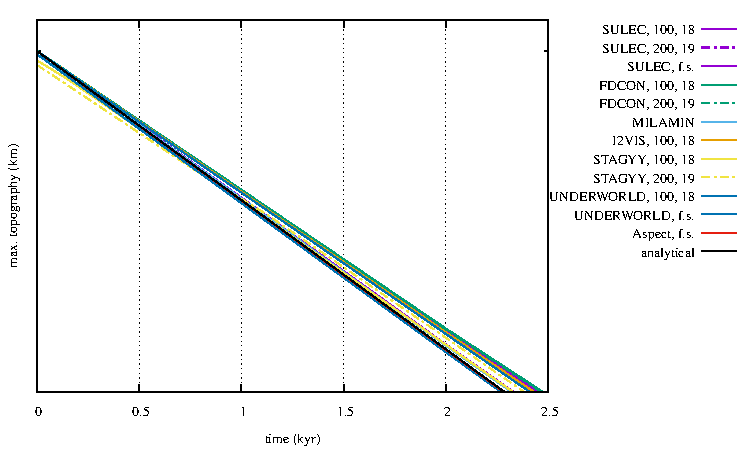
\includegraphics[width=7.5cm]{images/benchmark_crsg12/topozoom2.pdf}\\
{\captionfont Data from the original paper. Aspect data are obtained by running the available example in the code. }
\end{center}
